\section{Correctness evidence and independent geometric audit}
\label{sec:validation}

The mathematical bounds follow from the proofs, not from tests. The
experimental work checks the implementation, the normal-arc conventions,
source binding, exceptional topology, and the actual cost of the proposed
representation. All inherited source files in the delivered snapshot were
checked against their Git blob identifiers at the pinned commit. This
verification includes the precise bytes of the runtime, test fixtures,
and relevant research sources.

\subsection{Focused tests and old/new regression}

The three new test modules contain 39 test methods: 14 for transversals,
12 for the histogram algebra, and 13 for geometric integration. They cover
substantially more individual generated cases than the method count:
\begin{itemize}
\item 750 random finite interval systems under both periodic rules give
1,500 comparisons with an independent expanded least-representative oracle,
plus independent certificate replays and schedule-agreement checks.
\item 6,561 small type spectra and 729 doubling-chain spectra exercise
recovery and complete forward checking. Separate tests cover torus/Klein
zero-signature mixtures, impossible types, extraneous cover support, and
large exact integer fields.
\item Geometric tests cover layered meridians, several boundary vertices,
sphere/disc/M\"obius mixtures, projective planes, Klein bottles, pure vertex
links, boundary-edge inclusion, exact cycle allowances, source and proof
mutations, and early/late cancellation.
\item Large synthetic and geometric inputs use more than 20,000-bit
interval endpoints, 20,002-bit algebraic values, and 12,001-bit normal
multiplicities. They test encoded arithmetic without attempting an
expanded external oracle at those sizes.
\end{itemize}

The focused regression runner combines these additions with the relevant
existing interval, weighted-orbit, normal-surface, boundary, multiplicity,
component-census, and external-worker tests. It completes all 148 test
methods with zero failures, zero errors, and zero skips. This is the
specified geometry regression gate, not a claim that every unrelated
benchmark or every historical archive test in ProveIt was rerun. Exact
module names, raw output, runtime version and elapsed time are retained in
\path{results/regression_summary.json} and its companion log.

Mutation tests matter here because many false summaries preserve easy
invariants. A different set of representatives can have the right
cardinality. A wrong cover histogram can preserve total Euler weight.
Changing peeled vertex-link multiplicities can leave the query core
unchanged. The tests explicitly reject each of these changes through the
appropriate source-bound reconstruction step.

\subsection{External Regina oracle}

The frozen geometric corpus contains 664 surfaces on 34 labelled
triangulations, representing 26 triangulation isomorphism classes.
All are within the runtime's ambient contract. There are 630 nonempty
surfaces and 34 empty ones. Tetrahedron counts range from one to ten;
the largest coordinate is 85 and the largest explicit normal-disc count
is 1,528. These bounds keep the external oracle deliberately small.

The ambient examples include layered solid tori, boundary-cap variants,
an interior-vertex solid torus, projective-plane and Klein-bottle fixtures,
the trefoil and figure-eight exteriors, and exteriors of the torus knots
$T(2,5)$, $T(2,7)$, $T(3,4)$ and $T(3,5)$. Additional simplicial
relabelings exercise orientation and edge-order conventions. The sources
include selected Regina vertex vectors, bounded multiples, admissible sums
of compatible vectors, and distinguished fixtures. This is a diverse
constructed corpus, not a uniform random sample of all normal surfaces.

Regina 7.4 independently checks standard matching equations and
quadrilateral constraints, expands the bounded surface into connected
components, and queries each component's Euler characteristic, number of
boundary circles, and orientability. It verifies that component vectors
add to the original vector and that the additive invariants agree with
the whole surface. This procedure does not import the new producer's
geometry or reconstruction routines. Regina documents that these
particular component and boundary routines can expand discs or arcs
\cite{regina}; therefore it is used only as a bounded oracle, not as a
claimed compressed competitor on enormous coordinates.

Every case is processed by the direct and reduced APIs, and every tenth
case additionally uses the classical AHT periodic rule. The final audit
recomputes the Regina oracle afresh and checks every produced certificate.
The results are:

\begin{center}
\begin{tabular}{lr}
\toprule
Audit measure & Result\\
\midrule
Frozen source surfaces & 664\\
Direct census comparisons & 664\\
Quadrilateral-core census comparisons & 664\\
Additional classical-periodic-rule controls & 67\\
Exact external matches & 1,395\\
Successful independent certificate replays & 1,395\\
Failures or inconclusive results & 0\\
Distinct connected topological types & 49\\
Maximum orientable genus & 9\\
Maximum nonorientable crosscap number & 10\\
Maximum boundary circles on one component & 15\\
\bottomrule
\end{tabular}
\end{center}

The zero-signature test is geometric, not solely algebraic. A three-tetrahedron
orientable manifold with torus boundary and Regina isomorphism signature
\code{dHPabccdjw} contains the supplied closed Klein bottle. Its odd
multiples give mixtures of a Klein bottle and tori, all at the same
numerical key $(0,0)$. Both observer modes recover the distinct
orientability counts. Projective-plane and Klein-bottle fixtures test
the more general ambient contract; they are not asserted to be knot
exteriors in $S^3$.

The frozen corpus, provenance, oracle histograms, input-constructor hash,
runtime source hashes, canonical result hashes, and certificate hashes
are included. A portable replay uses the frozen answers without Regina;
an optional fresh replay recomputes the oracle. Both Python and Regina
generators are seeded, but the frozen face records are the authoritative
portable input because a random-number implementation can vary by platform.

\section{Paired performance measurements}
\label{sec:benchmarks}

\subsection{Question and comparison arms}

We measure the cost of obtaining the \emph{same full abstract type spectrum}
from a supplied validated-format input. The reference composition uses the
existing \code{normal\_component\_census}, with \code{mode="coordinates"}, to recover
each distinct component normal vector, and then the existing connected
topology query on each such vector. Their multiplicities are coalesced into
the same type rows. Its certificates retain the component-coordinate proof
and the individual topology proofs. This route computes extra embedding
information internally; it is an exact practical baseline, not an assertion
that every topology-only algorithm must pay for $7t$ coordinates.

The measured arms are the new direct two-weight query, an identical direct
A/A control, the new quadrilateral-core query, and that composed coordinate
reference. All produce certificates. Producer time and independent replay
time are measured separately, with their sum used for the principal paired
comparison. JSON serialization is outside those timed intervals; its exact
byte counts are measured separately. All arms must give the same spectrum,
and every certificate must verify.

The final protocol uses one untimed warm-up followed by five measured
rounds per case, with arm order shuffled from a recorded seed. Raw arm
orders and times are retained. The A/A arm quantifies ordinary timing
variation. The reported speedup is the median of within-round ratios of
producer-plus-replay time. Median milliseconds for each arm are also
shown; the ratio of those separate medians need not be identical to the
median paired ratio. These are observations on the recorded machine,
not complexity exponents or population-wide performance estimates.

\subsection{Families and exact expected spectra}

The dimension family uses primitive layered-solid-torus meridians at
$t=8,16,32,64,128$. The explicit number of normal discs grows with a
Fibonacci recurrence while the answer remains one disc. The direct
weighted dimension stays two; the coordinate reference uses $7t$.

The multiplicity family fixes a 16-tetrahedron meridian and uses
$x_g=gD+(g+1)L$ with $g=2^b$, for increasing exponent $b$.
Its full-coordinate gcd is one and its reduced query core is fixed.
One-sided families use the corresponding M\"obius-band and Klein-bottle
constructions, including odd/even M\"obius multiplicities and an odd
Klein-bottle multiplicity. A final family combines a M\"obius band with
both boundary-vertex discs and interior-vertex spheres. Pure vertex links
exercise the zero-query branch in the correctness tests. A separate
post-measurement check constructs the exact expected spectra from the
geometric scaling formulas and compares them to every recorded arm; these
calculations are outside the timed query.

\subsection{Final measurements}
The recorded environment is Python 3.12.14 on Linux x86\_64 with glibc 2.39.
The run on 9 October 2026 took approximately 183 seconds, including fixture
construction and out-of-timer serialization. All 260 measured calls and 52
warm-up calls completed; all result spectra agreed and all certificates
verified. Source hashes before and after the run agree. A separate formula
audit checks all 312 result hashes and the 52 retained proof summaries.

\begin{table}[H]
\centering\small
\begin{tabular}{rrrrrr}
\toprule
$t$ & $B$ & Reference (ms) & Direct (ms) & Core (ms) & Ref./direct\\
\midrule
8 & 6 & 14.543 & 8.421 & 8.487 & 1.745$\times$\\
16 & 11 & 57.406 & 23.569 & 23.080 & 2.430$\times$\\
32 & 22 & 299.345 & 84.474 & 93.117 & 3.446$\times$\\
64 & 44 & 1,981.496 & 424.342 & 424.830 & 4.763$\times$\\
128 & 89 & 14,912.555 & 2,662.092 & 2,581.826 & 5.733$\times$\\
\bottomrule
\end{tabular}
\caption{Primitive layered meridians. Times are medians of producer plus
independent replay. The final column is a median of paired ratios.}
\label{tab:dimension}
\end{table}

\begin{figure}[H]
\centering
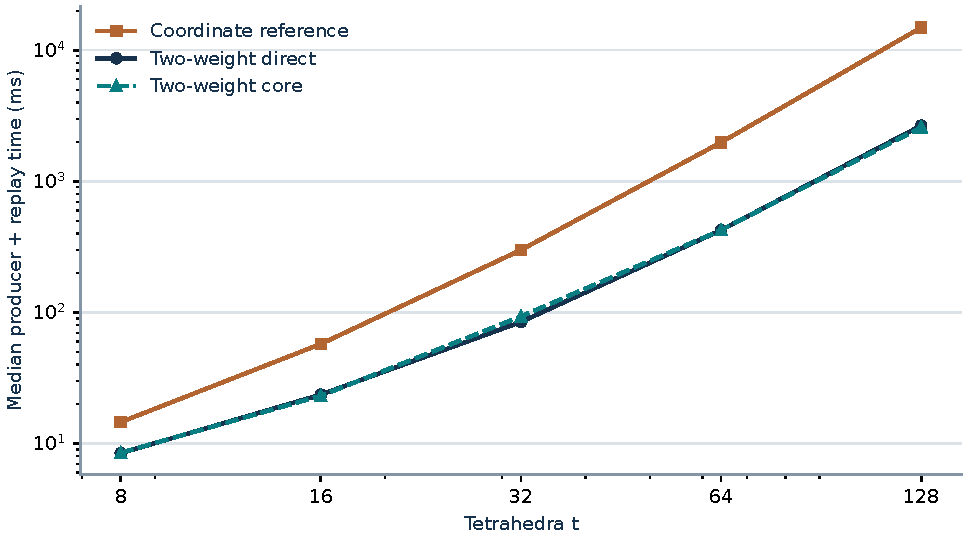
\includegraphics[width=\linewidth]{figures/dimension_timing.pdf}
\caption{Observed dimension-family timings, on logarithmic axes. Connecting
segments guide the eye; they are not fitted asymptotic laws. Core and direct
curves nearly coincide because these vectors have no large removable content.}
\label{fig:dimension}
\end{figure}

At $t=128$, the direct and coordinate-reference medians are approximately
2.662 and 14.913 seconds. The paired reference/direct factor is 5.733.
The corresponding serialized certificates contain 3,579,367 and 6,082,406
bytes. Thus this family shows increasing practical benefit from the smaller
observer, including a particularly large reduction in coordinate-reference
verification work. It does not identify a universal exponent in $t$.

\begin{table}[H]
\centering\small
\begin{tabular}{rrrrrr}
\toprule
Exponent $b$ & Input $B$ & Reference (ms) & Direct (ms) & Core (ms) & Direct/core\\
\midrule
128 & 139 & 126.738 & 52.977 & 22.972 & 2.322$\times$\\
4,096 & 4,107 & 161.687 & 90.527 & 24.942 & 3.631$\times$\\
16,384 & 16,395 & 212.546 & 193.630 & 27.738 & 6.994$\times$\\
32,768 & 32,779 & 299.004 & 331.892 & 32.055 & 10.368$\times$\\
\bottomrule
\end{tabular}
\caption{Fixed $16$-tetrahedron core with $g=2^b$ and
$x_g=gD+(g+1)L$. All full-coordinate gcds are one.}
\label{tab:multiplicity}
\end{table}

\begin{figure}[H]
\centering
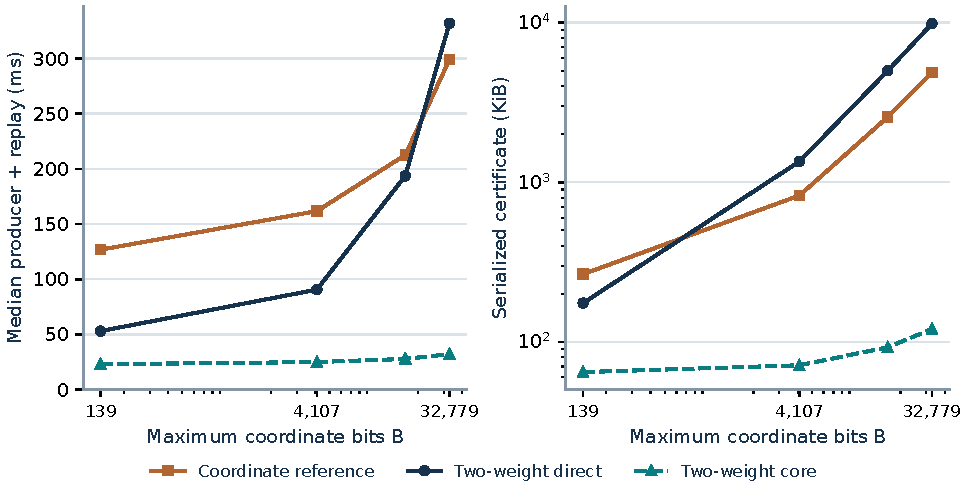
\includegraphics[width=\linewidth]{figures/multiplicity_timing_and_proofs.pdf}
\caption{The fixed-core family: observed time and certificate size.
Only the orbit-query core becomes small; original source coordinates,
divisor and restored binary multiplicities still appear in the computation.}
\label{fig:multiplicity}
\end{figure}

For the largest fixed-core input, with $B=32,779$, the direct and core
medians are 331.892 and 32.055 milliseconds; the paired improvement is
10.368. The certificates shrink from 10,081,806 to 123,278 bytes, a factor
of about 81.78. The reduced proof therefore remains dependent on $B$, as
predicted, but avoids repeating large multiplicities throughout the orbit
trace. Serialized size is not peak resident memory: the latter was not
measured.

\begin{table}[H]
\centering\small
\begin{tabular}{lrrrr}
\toprule
Family & Reference (ms) & Direct (ms) & Core (ms) & Direct/core\\
\midrule
M\"obius, even & 2.857 & 3.021 & 0.881 & 3.513$\times$\\
M\"obius, odd & 3.354 & 3.098 & 0.889 & 3.458$\times$\\
Klein, odd & 8.320 & 7.678 & 1.553 & 4.672$\times$\\
M\"obius + sphere/disc links & 13.149 & 10.391 & 2.089 & 4.973$\times$\\
\bottomrule
\end{tabular}
\caption{One-sided and mixed-link families at exponent 4,096. These include
parity restoration and the closed zero-signature collision.}
\label{tab:one-sided}
\end{table}

There are informative negative comparisons. On the $b=32,768$ meridian
mixture, the unreduced direct query is slower than the coordinate reference:
their median times are 331.892 versus 299.004 milliseconds, with a paired
reference/direct ratio of 0.900. The even M\"obius example similarly gives
a ratio of 0.945. The core mode is faster on both examples. On a primitive
$t=32$ meridian, reduction increases the median from 84.474 to 93.117
milliseconds; the paired direct/core ratio is 0.912. These measurements
support an explicit choice of representation, not a universal replacement
claim.

Across all cases, the paired A/A ratios range from 0.915 to 1.028. Five repeats are adequate for a transparent exploratory comparison, but do not establish statistical significance for small differences. No confidence interval, runtime-exponent fit, whole-knot speedup, or extrapolation to untested hard diagrams is claimed. The complete per-phase times, orders, exact inputs and proof hashes are in the raw JSON; the accompanying CSV exposes every reported median.



\subsection{Interpretation and limits of the measurements}

The growing-dimension family isolates the benefit of avoiding coordinate
recovery and per-component topology reconstruction. The fixed-core families
isolate the cost of carrying large multiplicities through each local event.
They support the parameter-sensitive claims in
\cref{thm:transversal,thm:census,thm:core}, but are not a random corpus of
hard knot diagrams. The code contains no new end-to-end diagram recognizer,
so none of these speedup factors should be advertised as an unknot-recognition
speedup from planar diagram input.

Primitive instances have almost nothing to remove. The reduced mode adds
gcd, minima, division and core validation work, so small slowdowns or
differences within the A/A variation are expected and reported. The
constant-dimensional observer is not uniformly faster on every possible
input: marker complexity, trace geometry, and how much extra component
information is needed all affect the comparison.

Reducing a fixed core removes outer multiplicities from orbit endpoints,
but the full call and the outer proof still contain and process their
binary representations. The timings establish actual implementation gains;
they do not establish a smaller exponent of the total bit-complexity
polynomial on a fixed-core family.

\section{Reproduction and delivered artifacts}
\label{sec:reproduce}

The archive includes this article and its complete LaTeX source, the six
new modules, a pinned runnable code snapshot, integration patch, focused
tests and fixtures, external corpus and audit, benchmark driver and raw
measurements, retained benchmark proofs, plotting code and figures, and
file/source manifests. Existing third-party papers are referenced by URL
and are not redistributed. The inherited code licence is retained.

From \path{code/fast}, the principal commands are:
\begin{lstlisting}
python3 topology_research/run_tests.py --output local_results

python3 topology_research/regina_audit.py audit \
  --corpus topology_research/data/regina_corpus.json \
  --output local_results/regina_replay.json

python3 topology_research/regina_audit.py audit \
  --corpus topology_research/data/regina_corpus.json \
  --output local_results/regina_fresh.json --recheck-oracle
\end{lstlisting}
The second command replays frozen independently obtained answers without
requiring Regina; the third needs Regina and rebuilds each bounded oracle
answer. The benchmark driver exposes its parameters through \code{--help};
the recorded configuration and an equivalent explicit invocation are retained
in the results and package README.
The outer \code{reproduce.py} script offers the focused regression gate,
frozen audit, and article build as separate reproducible steps.

The integration patch is additive and should first be checked against the
target checkout with \code{git apply --check}. The pinned snapshot enables
reproduction even if main changes after this report. Reusing an earlier
result JSON without matching runtime hashes is not an equivalent measurement.
